\section{Численные эксперименты}
\label{sec:Chapter4} \index{Chapter4}

% \subsection{Тест 1}
\par Тесты производились на интересующей нас задаче – линейной системе с многими 
правыми частями, возникающей при решении задачи электромагнитного рассеяния 
методом интегральных уравнений [STAVTSEV]. Порядок системы - 14144, всего правых частей - 722.
\begin{figure}[H]
    \centering
    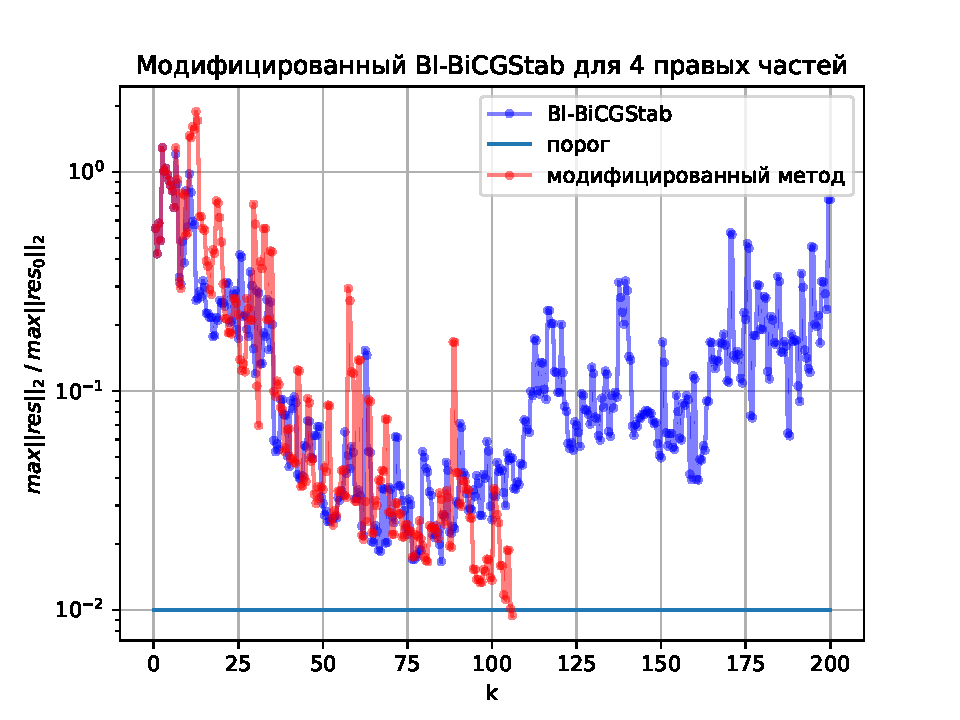
\includegraphics[width=0.7\linewidth]{images/4.pdf}
    \caption{}
    \label{fig:4}
\end{figure} 
\par Первый тест демонстрирует, что метод из статьи [GUENNOUNI] не сходится с требуемой точностью, в то время как 
версия с улучшениями, описанными в главе \ref{sec:Chapter3}, сходится линейно без проблем. 
Эксперимент проводился в одинарной точности для четырех правых частей с номерами: 0, 90, 180, 270. Его результаты представлены
на рис.\ref{fig:4}
% \subsection{Тест 2}
\begin{figure}[H]
    \centering
    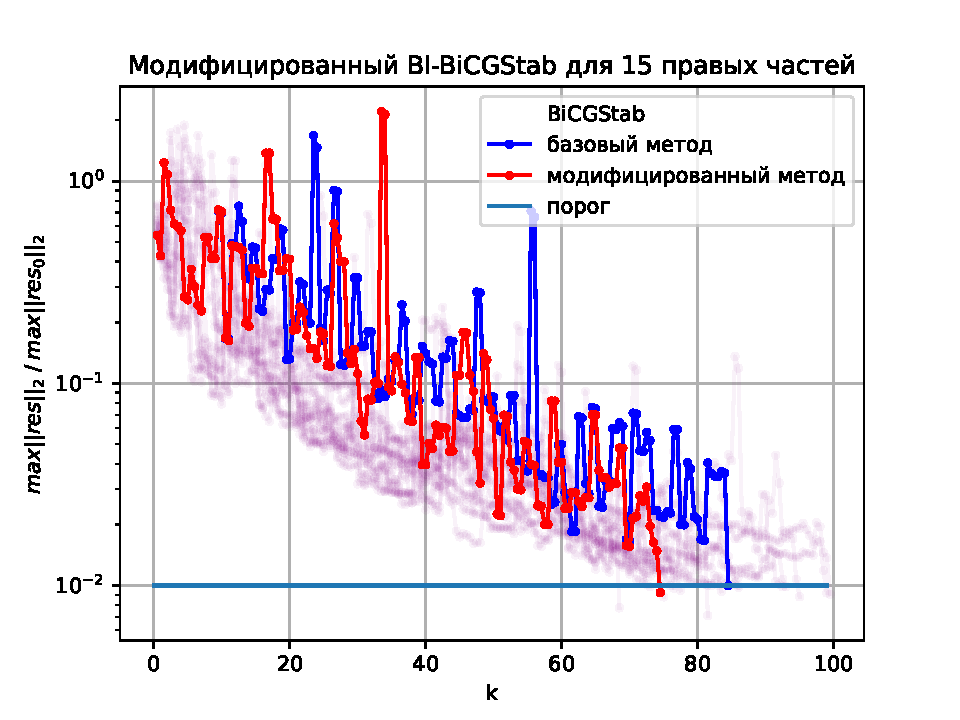
\includegraphics[width=0.7\linewidth]{images/acceleration_15_rhs.pdf}
    \caption{}
    \label{fig:acceleration_15}
\end{figure}
\par 15 правых частей, уменьшения числа итераций, считаем в двойной точности
\par Второй тест демонстрирует, что улучшения, описанные в главе \ref{sec:Chapter3} позволяют получить выгоду по количеству матвеков,
по сравнению с решением систем с каждой правой частью в отдельности. Эксперимент проводился в двойной точности с 15 правыми частями,
выбранными с помощью RRQR. Его результаты представлены на рис.\ref{fig:acceleration_15}. По оси абцисс - количество иттераций, по оси
ординат - относительная максимальная невязка в блоке. Фиолетовым изображено падение невязки при решении задачи с каждой правой частью 
в отдельности, синим - метод из статьи [GUENNOUNI], красным - метод с улучшениями из главы \ref{sec:Chapter3}. Для решения этой задачи
стабилизированными бисопряженными градиентами было потрачено 2525 матвеков, для решения методом из статьи [GUENNOUNI] - 2535, модифицированный
метод сошелся за 2235 матвеков, таким образом выгода составляет 12\% по сравнению с неблочной версией.
% \subsection{Тест 3}
\par более 30 правых частей, демонстрация отсутствия взрыва невязки
\begin{figure}[H]
    \centering
    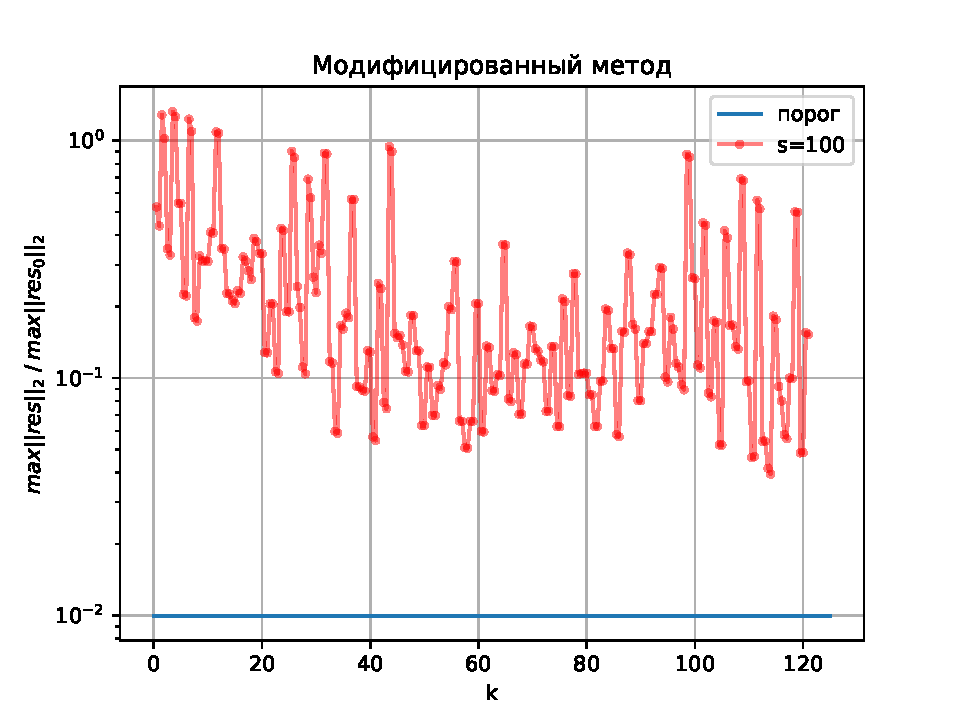
\includegraphics[width=0.7\linewidth]{images/100_rhs.pdf}
    \caption{}
    \label{fig:100_rhs}
\end{figure}

\newpage
